At first we removed the images from the data-set where the pose was too much away from frontal.\\
For doing the pre-processing we first figure out the centre of the two eyes using eye-detectors and then we align such that two eye centres are parallel to the x-axis of the image(so that the image looks frontal even if the face is tilted to some extent) and resize the faces so that distance between the two eyes is 128 pixels and the image size is $256\times 256$. We don't keep the whole image but just the face which is recognised by the detector.\\ \\
First we define the align and resize function which takes in the eye centre co-ordinates and results out the output image which is aligned, cropped and resized.

\begin{lstlisting}[style=Python]
    def align_eye(self, image, leftEyeCenter, rightEyeCenter):
		dY = rightEyeCenter[1] - leftEyeCenter[1]
		dX = rightEyeCenter[0] - leftEyeCenter[0]
		angle = np.degrees(np.arctan2(dY, dX)) - 180
		desiredRightEyeX = 1.0 - self.desiredLeftEye[0]

		dist = np.sqrt((dX ** 2) + (dY ** 2))
		desiredDist = (desiredRightEyeX - self.desiredLeftEye[0])
		desiredDist *= self.desiredFaceWidth
		scale = desiredDist / dist

		eyesCenter = ((leftEyeCenter[0] + rightEyeCenter[0]) // 2, \
		(leftEyeCenter[1] + rightEyeCenter[1]) // 2)

		M = cv2.getRotationMatrix2D(eyesCenter, angle, scale)

		tX = self.desiredFaceWidth * 0.5
		tY = self.desiredFaceHeight * self.desiredLeftEye[1]
		M[0, 2] += (tX - eyesCenter[0])
		M[1, 2] += (tY - eyesCenter[1])

		(w, h) = (self.desiredFaceWidth, self.desiredFaceHeight)
		output = cv2.warpAffine(image, M, (w, h), flags=cv2.INTER_CUBIC)
		return output
\end{lstlisting}

Here given the desired distance between the two eyes and the image we find out the transformation matrix which rotates and resizes the image so that the distance between the two eyes is 128 pixels. It rotates the image in such a way that the two eyes are in parallel to x-axis of the image.
\newpage
For figuring out the location of left and right eye we use two different methods:
\begin{itemize}
    \item \textbf{HARR face and eye detectors}\\
    Here we use HARR cascade classifier to figure out the the face in the image and then crop out the face. We then use the eye classifier to figure out the eye from the cropped image.
    
    \begin{lstlisting}[style=Python]
    face_cascade = cv2.CascadeClassifier('./haarcascades/haarcascade_\
frontalface_default.xml')
    eye_cascade = cv2.CascadeClassifier('./haarcascades/haarcascade_eye.xml')
    for i in range(self.n):
	img = self.data[i]
	img_gray = gray[i]
			
	try:
	    faces = face_cascade.detectMultiScale(img_gray, 1.3, 5)
	    (x,y,w,h) = faces[0]
	    roi_gray = img_gray[y:y+h, x:x+w]
		roi_color = img[y:y+h, x:x+w]
				
		eyes = eye_cascade.detectMultiScale(roi_gray, 1.1, 3)
		(ex1,ey1,ew1,eh1) = eyes[0]
		(ex2,ey2,ew2,eh2) = eyes[1]
				
		if(ex1 < ex2):
		    lt_mid = [(ex1+(int)(ew1/2)), (ey1+(int)(eh1/2))]
		    rt_mid = [(ex2+(int)(ew2/2)), (ey2+(int)(eh2/2))]
		else:
		    rt_mid = [(ex1+(int)(ew1/2)), (ey1+(int)(eh1/2))]
		    lt_mid = [(ex2+(int)(ew2/2)), (ey2+(int)(eh2/2))]
	except:
		print("    "+str(i+1)+" failed")
		continue
	print("    "+str(i+1))
	res.append(fa.align_eye(roi_color, rt_mid, lt_mid))
    \end{lstlisting}
    Here in some images the classifier is not able to figure out the eyes or the face for that we have used try and except. In this for about 65\% images it works fine and for others out of 20 images only 8-13 images can be figured out, for images folder names "Suraj" the classifier couldn't figure out even a single image.
    
    \item \textbf{Dlib face detector}
    We tried using dlib's face detectors which detects out the face, eyes, noes, etc. from the face image.
    \begin{lstlisting}[style=Python]
    detector = dlib.get_frontal_face_detector()
    predictor = dlib.shape_predictor("shape_predictor_68_face_landmarks.dat")
    \end{lstlisting}
    We use the above predictor to figure out the eyes centre and then gave that to our align\_eye function defined above which gives out the aligned and cropped output image. Applying this worked for almost 80\% of all the images. But, again for images in folder named "Suraj" it couldn't figure out even a single image. We even tried just figuring out the face out of the image using Harr face classifier but didn't worked for "Suraj".
\end{itemize}
We save the pre-processed image to use them to train our model. \\
Some result from the above pre-processing:

\begin{figure}[!h]
    \centering
    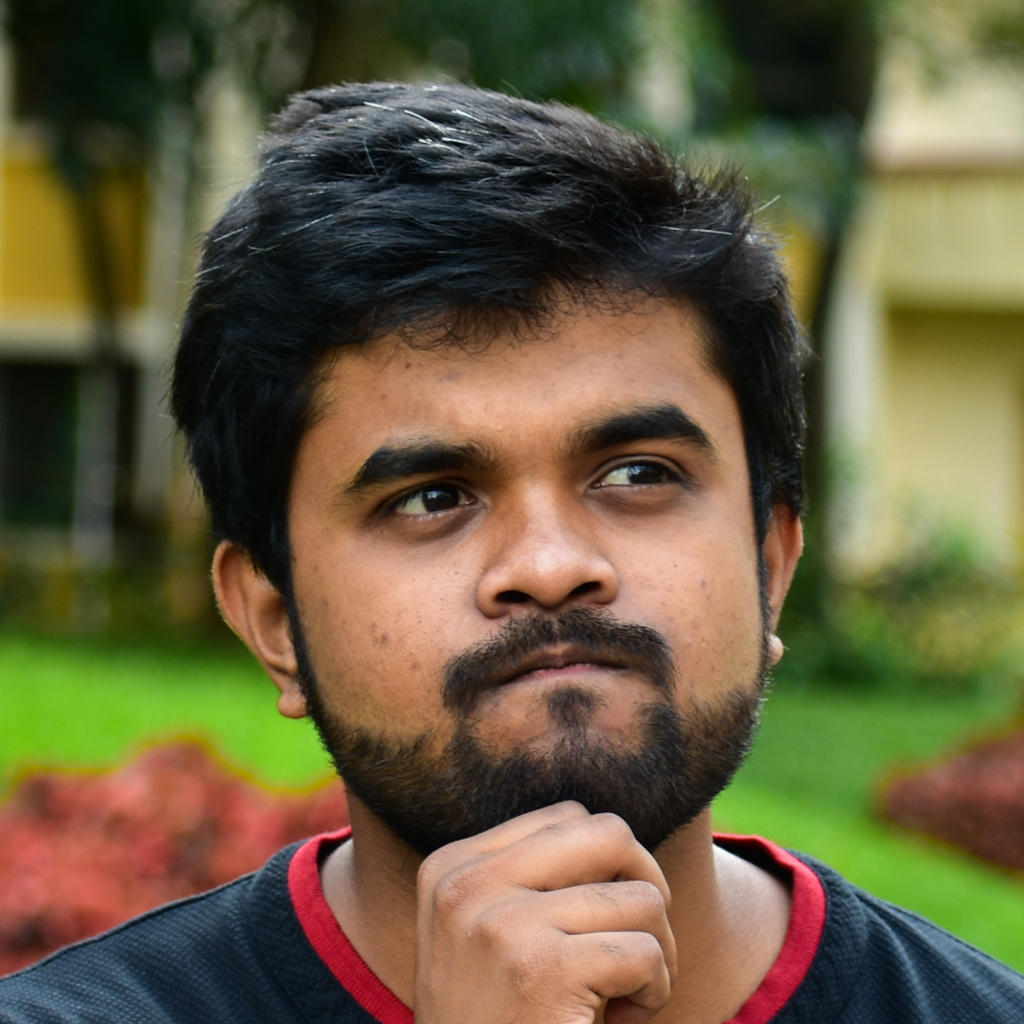
\includegraphics[width=0.3\linewidth]{image.jpg}
    \caption{Image}
    \label{fig1}
\end{figure}


\begin{figure}[!htb]
    \minipage{0.32\textwidth}
      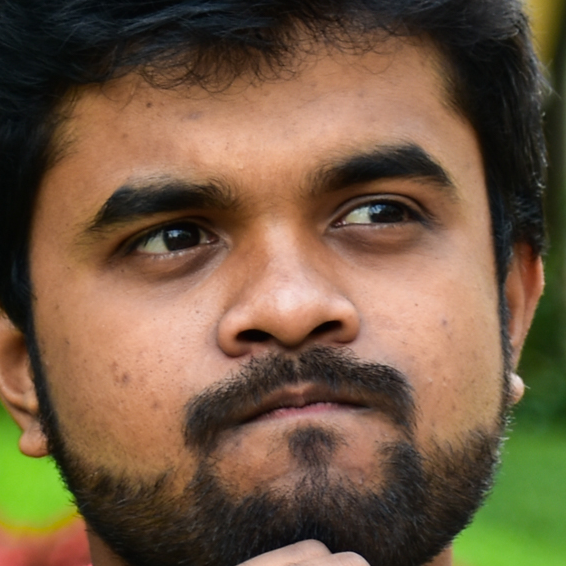
\includegraphics[width=\linewidth]{Harr.png}
      \caption{Harr(only face)}\label{fig2}
    \endminipage\hfill
    \minipage{0.32\textwidth}
      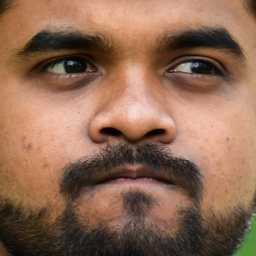
\includegraphics[width=\linewidth]{Harr_eye.png}
      \caption{Harr(face and eye)}\label{fig3}
    \endminipage\hfill
    \minipage{0.32\textwidth}%
      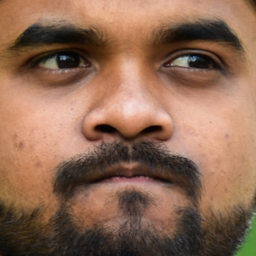
\includegraphics[width=\linewidth]{dlib.png}
      \caption{dlib}\label{fig4}
    \endminipage
\end{figure}

We can clearly see that the face in Figure \ref{fig1} is slightly tilted, this can also be seen when we pre-process by using Harr detectors with only face detectors which just crop out the face from the image(Figure \ref{fig2}). After that when we use Harr with eye detectors or dlib which also detect eye centre and then realign the images we can see the face does not looks tilted (Figure \ref{fig3} and Figure \ref{fig4})